\section{Introduction}
\label{sec:introduction}

%{\color{blue} In this section we will contextualize video streaming technology and hierarchical caching problems, emphasizing the need of create a hierarchical topology to , and describe the content of each section of the paper.}

% Introduction of the Content and MEC service provider  
Over the years, the Internet traffic has growing exponentially around the world. Mainly, due to the multimedia content streaming which, currently, represents the 70\% of the whole traffic. To delivery a video, the streaming is generated by Video-on-Demand services and distributed by the the Over-The-top providers, while they attempt to satisfy the quality of experience~(QoE) to a wide range of users subscribers. To provide the best user satisfaction, OTT providers may take advantages of the high data-rate and low-latency in the edge network~\cite{DBLP:CoRR:2021}. In this way, caching the video closer to the end-user has a positive impact in the QoE performances.

% Challenges
The advantages of using the edge of the network to store the video helps in user satisfaction but could has negative impact as well. Since the triggered video segments caching (replication) in a edge node
However, there are certain precautions when choosing the nodes for caching the video that need to be taken into account. 

\begin{figure}
    \centering
    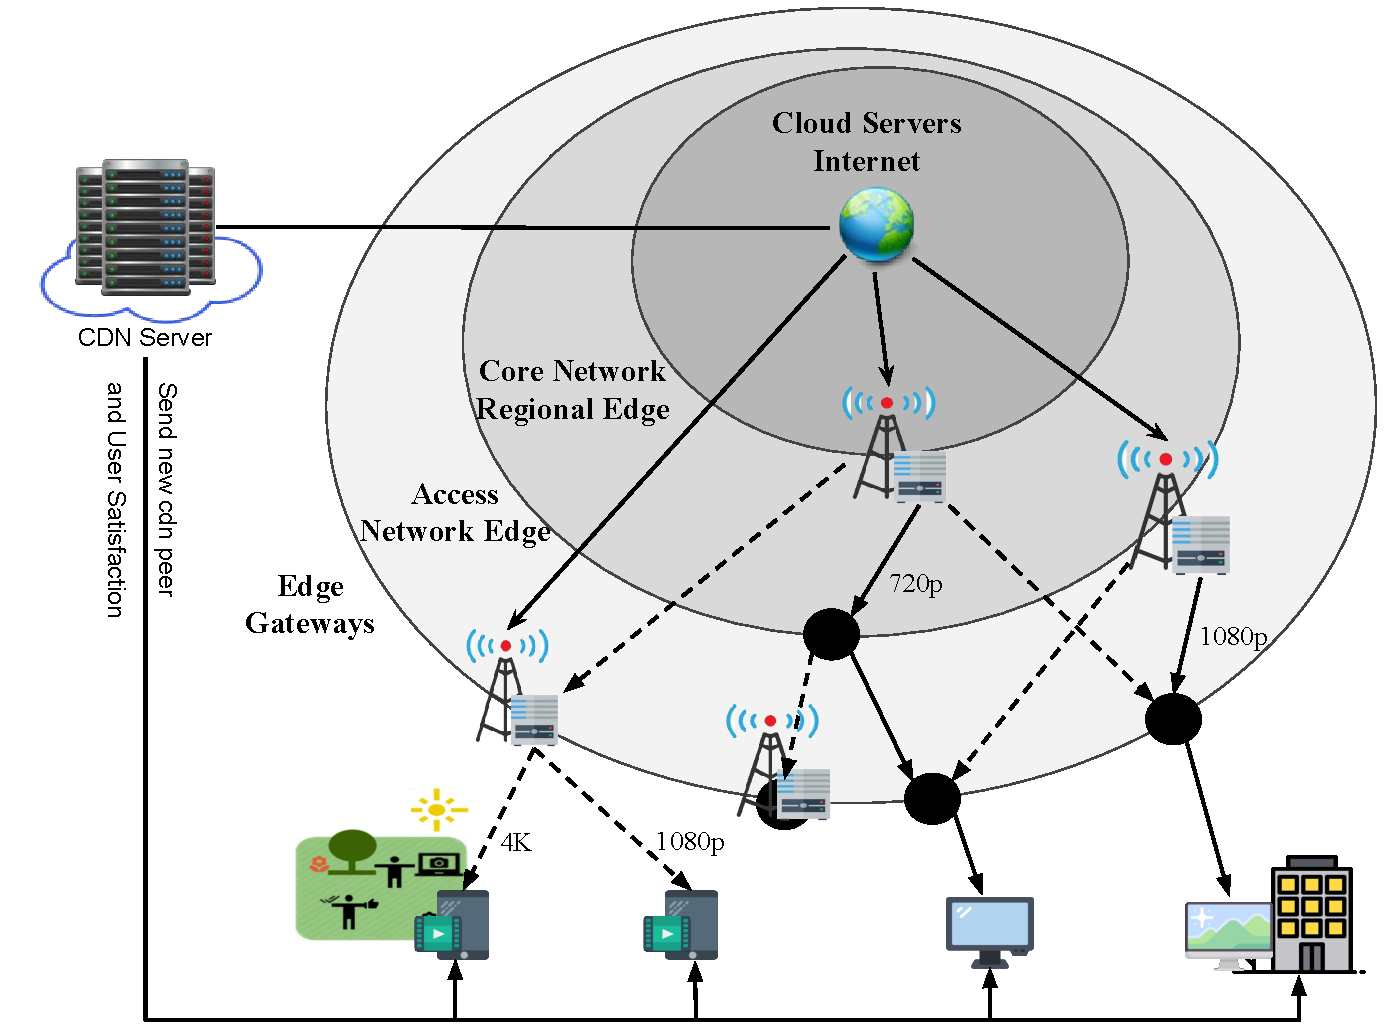
\includegraphics[width=0.9\linewidth]{images/arch-video-content.pdf}
    \caption{A General Overview of the multi-tier network environment.}
    \label{fig:impact-two-layers}
\end{figure}

Nowadays, When a large number of users start to request video segments at the edge nodes, this surrogated nodes considers the static users and just one edge nodes tiers. Which it could result some issues. 

% Objective
Motivated by the advantages of multi-level fog/cloud scenarios to improve user satisfaction, as well as video traffic grows exponentially. This article presents the need to have an orchestrator for the provision of video streaming content.
. Our goal is to provide designers and operators an performance analysis  of an hierarchical edge network and its impacts on the users' QoE. The models we present in this paper are evaluated by a series of simulations using a controlled environment.

% Organization paper
This work is organized as follows.
Section \ref{sec:related-work} presents related work on the impact of edge/cloud network on video streaming services.
Section \ref{sec:system-archi} briefly describes the proposed muti-tier edge/cloud network.
Section \ref{sec:results} shows a preliminarly results on the impact of the network performance for video streaming services.
Finally, \ref{sec:conclusion} concludes the paper.